\documentclass[11pt,a4paper]{article}

% ============================================================
% Packages
% ============================================================
\usepackage[margin=1in]{geometry}
\usepackage{amsmath,amssymb,mathtools}
\usepackage{booktabs}
\usepackage{array}
\usepackage{longtable}
\usepackage{multirow}
\usepackage{graphicx}
\usepackage{xcolor}
\usepackage{tikz}
\usepackage{pgfplots}
\usepackage{pgfplotstable}
\usepackage{hyperref}
\usepackage{float}
\usepackage{enumitem}
\usepackage{microtype}
\usepackage{siunitx}
\usepackage{adjustbox}

\usetikzlibrary{
    arrows.meta,
    positioning,
    shapes.geometric,
    shapes.misc,
    fit,
    backgrounds,
    calc
}

\pgfplotsset{compat=1.18}

% ============================================================
% Colors
% ============================================================
\definecolor{gpuBlue}{RGB}{50,110,190}
\definecolor{gpuDark}{RGB}{30,65,120}
\definecolor{energyGreen}{RGB}{40,145,90}
\definecolor{latencyRed}{RGB}{205,65,65}
\definecolor{frameworkPurple}{RGB}{120,75,170}
\definecolor{lightblue}{RGB}{235,244,255}
\definecolor{lightgreen}{RGB}{235,250,241}
\definecolor{lightred}{RGB}{255,239,239}
\definecolor{lightpurple}{RGB}{245,238,255}
\definecolor{graybox}{RGB}{242,242,242}

% ============================================================
% Hyperref
% ============================================================
\hypersetup{
    colorlinks=true,
    linkcolor=gpuDark,
    citecolor=frameworkPurple,
    urlcolor=gpuBlue
}

% ============================================================
% Custom commands
% ============================================================
\newcommand{\framework}[1]{\textbf{#1}}
\newcommand{\unknown}{\textemdash}
\newcommand{\tokps}{\mathrm{tokens/s}}
\newcommand{\jptok}{\mathrm{J/token}}
\newcommand{\ttft}{\mathrm{TTFT}}
\newcommand{\itl}{\mathrm{ITL}}

% ============================================================
% Title
% ============================================================
\title{
    \textbf{Efficient AI Inference Frameworks}\\[0.4em]
    \large Energy Efficiency, Token Throughput, Latency,
    Architecture, and Capability Overview
}

\author{Technical Survey}
\date{2026}

\begin{document}

\maketitle

\begin{abstract}
This document surveys efficient AI inference frameworks, runtimes,
serving systems, and compiler stacks, including several relatively
niche projects.  The primary objective is to understand how modern
AI inference systems improve token throughput, latency, memory
efficiency, and energy efficiency.

Twenty-four systems are compared, including vLLM, SGLang,
TensorRT-LLM, llama.cpp, MLX, MLC-LLM, CTranslate2, mistral.rs,
ExLlamaV3, OpenVINO, ONNX Runtime, IREE, ExecuTorch, Candle,
DeepSpeed-MII, Aphrodite Engine, LMDeploy, TGI, Triton Inference
Server, FasterTransformer, XLA/JAX, TVM, ggml, and AWS Neuron.

A critical distinction is made between \emph{measured benchmark
results} and \emph{framework capabilities}.  Publicly available
benchmarks do not currently provide an apples-to-apples energy-per-
token measurement for all systems.  Consequently, this document
does not invent such measurements.  Instead, it provides a rigorous
method for measuring joules per generated token and includes plots
for the publicly reported throughput and latency measurements that
are available.
\end{abstract}

\tableofcontents
\newpage

% ============================================================
\section{Executive Overview}
% ============================================================

Modern AI inference is not determined solely by the neural-network
model.  The runtime surrounding the model can substantially change
how effectively hardware is utilized.

A simplified inference pipeline is:

\[
\boxed{
\text{Request}
\rightarrow
\text{Tokenizer}
\rightarrow
\text{Scheduler}
\rightarrow
\text{Prefill}
\rightarrow
\text{KV Cache}
\rightarrow
\text{Decode}
\rightarrow
\text{Sampler}
\rightarrow
\text{Output}
}
\]

The main optimization targets are:

\begin{align}
\text{Throughput} &=
\frac{\text{generated tokens}}{\text{second}},\\[4pt]
\text{Energy efficiency} &=
\frac{\text{generated tokens}}{\text{joule}},\\[4pt]
\text{Energy/token} &=
\frac{\text{joules consumed}}{\text{generated tokens}},\\[4pt]
\text{TTFT} &=
\text{time to first generated token},\\[4pt]
\text{ITL} &=
\text{inter-token latency}.
\end{align}

A framework that maximizes throughput does not necessarily minimize
joules per token.  Similarly, a framework that minimizes TTFT does
not necessarily maximize aggregate throughput.

Therefore:

\[
\boxed{
\text{Best framework}
\neq
\text{universally fastest framework}
}
\]

Instead:

\[
\boxed{
\text{Optimal system}
=
f(
\text{model},
\text{hardware},
\text{batch},
\text{context},
\text{quantization},
\text{traffic},
\text{latency target}
)
}
\]

Recent same-hardware tests demonstrate exactly this workload
dependence.  For example, one Qwen3-32B benchmark measured
different throughput and TTFT behavior for vLLM, SGLang, and
TensorRT-LLM as concurrency and context length changed
\cite{benchmark2026}.

% ============================================================
\section{How an AI Inference Framework Works}
% ============================================================

\subsection{High-Level Architecture}

\begin{figure}[H]
\centering

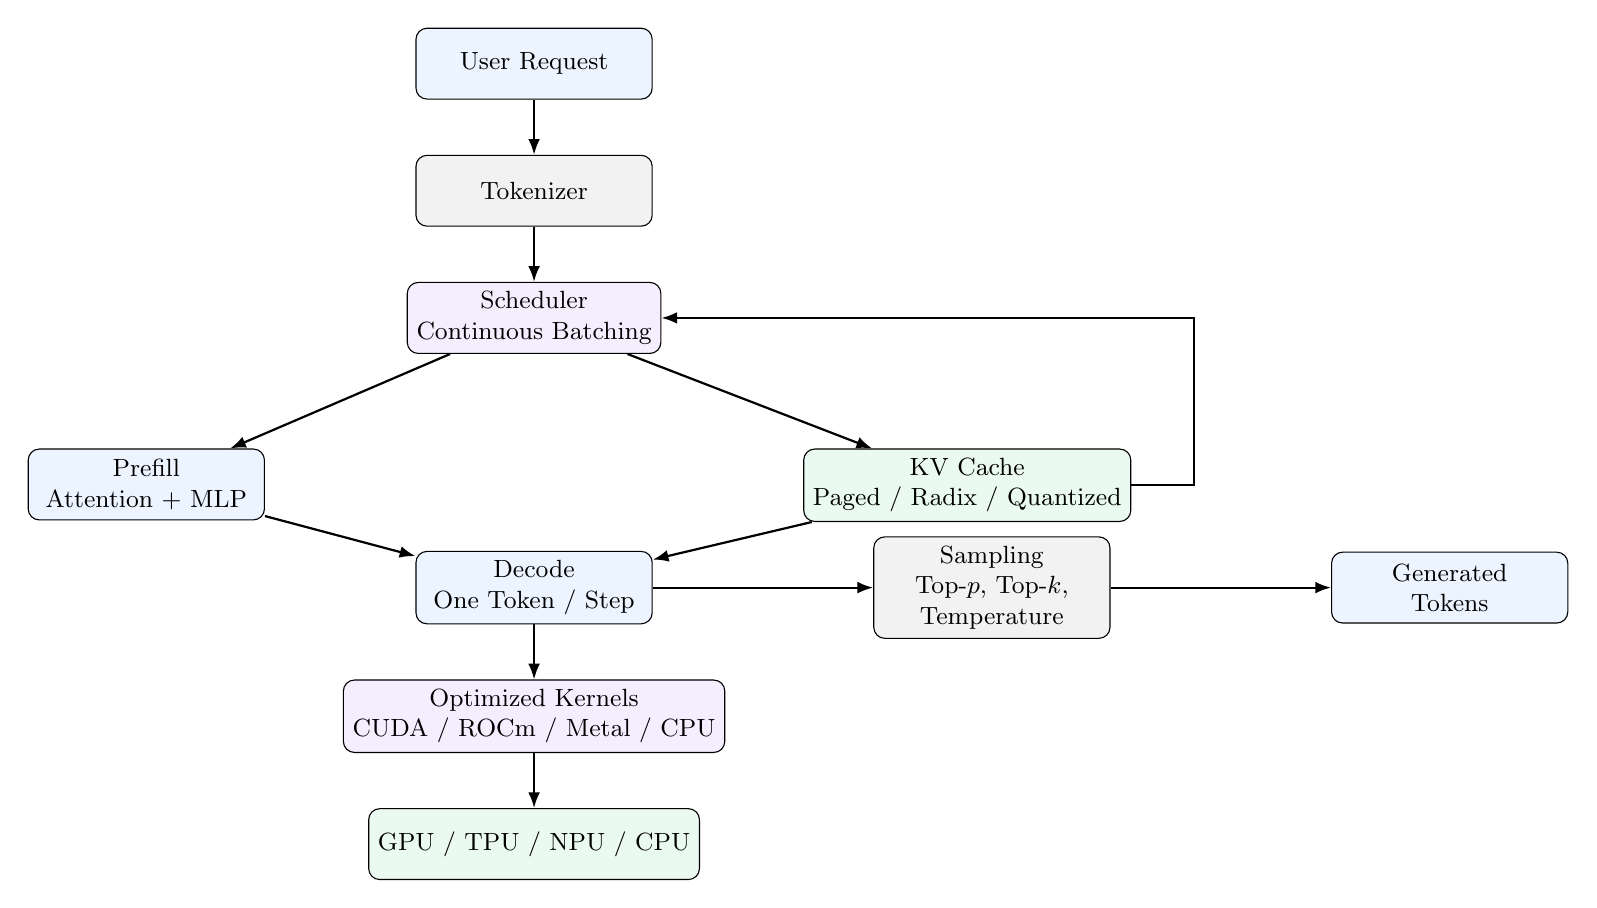
\begin{tikzpicture}[
    node distance=7mm and 10mm,
    box/.style={
        draw,
        rounded corners,
        minimum width=30mm,
        minimum height=9mm,
        align=center,
        font=\small
    },
    arrow/.style={
        -{Latex[length=2mm]},
        thick
    }
]

\node[box, fill=lightblue] (request)
    {User Request};

\node[box, fill=graybox, below=of request] (tokenizer)
    {Tokenizer};

\node[box, fill=lightpurple, below=of tokenizer] (scheduler)
    {Scheduler\\Continuous Batching};

\node[box, fill=lightblue, below left=12mm and 18mm of scheduler]
    (prefill)
    {Prefill\\Attention + MLP};

\node[box, fill=lightgreen, below right=12mm and 18mm of scheduler]
    (kv)
    {KV Cache\\Paged / Radix / Quantized};

\node[box, fill=lightblue, below=25mm of scheduler]
    (decode)
    {Decode\\One Token / Step};

\node[box, fill=lightpurple, below=of decode]
    (kernel)
    {Optimized Kernels\\CUDA / ROCm / Metal / CPU};

\node[box, fill=lightgreen, below=of kernel]
    (hardware)
    {GPU / TPU / NPU / CPU};

\node[box, fill=graybox, right=28mm of decode]
    (sampler)
    {Sampling\\Top-$p$, Top-$k$,\\Temperature};

\node[box, fill=lightblue, right=28mm of sampler]
    (output)
    {Generated\\Tokens};

\draw[arrow] (request) -- (tokenizer);
\draw[arrow] (tokenizer) -- (scheduler);
\draw[arrow] (scheduler) -- (prefill);
\draw[arrow] (scheduler) -- (kv);
\draw[arrow] (prefill) -- (decode);
\draw[arrow] (kv) -- (decode);
\draw[arrow] (decode) -- (kernel);
\draw[arrow] (kernel) -- (hardware);
\draw[arrow] (decode) -- (sampler);
\draw[arrow] (sampler) -- (output);

\draw[arrow] (kv.east) -| ++(8mm,0) |- (scheduler.east);

\end{tikzpicture}

\caption{Simplified architecture of an optimized AI inference
runtime.}
\end{figure}

% ============================================================
\section{Why Inference Is Difficult}
% ============================================================

For autoregressive language models, generation approximately follows

\[
P(x_1,\ldots,x_T)
=
\prod_{t=1}^{T}
P(x_t\mid x_{<t}).
\]

The model therefore generates tokens sequentially.

During decoding, a simplified computation is

\[
x_{t+1}
=
f_\theta(x_{\leq t},K_t,V_t).
\]

The KV cache stores previously computed key/value tensors:

\[
K_t =
[K_1,K_2,\ldots,K_t],
\qquad
V_t =
[V_1,V_2,\ldots,V_t].
\]

For long contexts and many concurrent users, KV-cache memory can
become one of the principal constraints.

This motivates several important optimization families:

\begin{enumerate}
    \item Paged KV caching.
    \item Continuous/in-flight batching.
    \item Prefix caching.
    \item Radix/tree-based attention caching.
    \item Quantization.
    \item Fused GPU kernels.
    \item CUDA graph execution.
    \item Speculative decoding.
    \item Tensor parallelism.
    \item Pipeline parallelism.
    \item Expert parallelism for MoE models.
    \item Disaggregated prefill/decode.
    \item Compiler-level graph optimization.
    \item Hardware-specific kernels.
\end{enumerate}

% ============================================================
\section{Major Optimization Techniques}
% ============================================================

\subsection{Paged KV Cache}

Instead of requiring a contiguous KV-cache allocation, memory can
be divided into pages:

\[
\mathrm{KV}
=
\bigcup_{i=1}^{N}\mathrm{page}_i.
\]

This allows memory to be dynamically allocated between requests.

Conceptually:

\[
\text{Request A}
\rightarrow
[P_1,P_4,P_7]
\]

\[
\text{Request B}
\rightarrow
[P_2,P_5,P_9]
\]

rather than requiring one large contiguous memory region.

This is one of the central ideas behind modern high-throughput
LLM serving systems.

\subsection{Continuous Batching}

Traditional batching waits for all requests in a batch:

\[
\boxed{
R_1,R_2,R_3
\rightarrow
\text{finish together}
}
\]

Continuous batching instead dynamically inserts and removes
requests:

\[
\boxed{
R_1,R_2
\rightarrow
R_3
\rightarrow
R_4
\rightarrow
R_5
}
\]

at the token-generation level.

This increases hardware utilization when request lengths vary.

\subsection{Prefix Caching}

If two requests share a prefix,

\[
P =
[\text{system prompt},\text{instructions},\text{context}],
\]

the runtime may reuse the corresponding KV states.

Thus:

\[
T_{\text{prefill}}
\rightarrow
T_{\text{prefill, uncached}}
\]

can become approximately

\[
T_{\text{prefill,cached}}
\ll
T_{\text{prefill, uncached}}.
\]

This is particularly valuable for agents, RAG systems, and repeated
system prompts.

\subsection{Quantization}

A model can be represented at different numerical precisions:

\[
\mathrm{FP32}
\rightarrow
\mathrm{FP16/BF16}
\rightarrow
\mathrm{FP8}
\rightarrow
\mathrm{INT8}
\rightarrow
\mathrm{INT4}.
\]

The theoretical memory requirement for parameters is approximately

\[
M
\approx
N_{\mathrm{params}}
\times
\frac{b}{8},
\]

where $b$ is the number of bits per parameter.

For a 70-billion parameter model:

\[
M_{\mathrm{FP16}}
\approx
70\times10^9
\times
\frac{16}{8}
=
140\ \mathrm{GB},
\]

before accounting for additional runtime memory.

% ============================================================
\section{Framework Landscape}
% ============================================================

The following table intentionally includes both full serving
frameworks and lower-level runtimes/compilers because the distinction
is important when discussing ``AI frameworks.''

\begin{longtable}{p{3.2cm} p{3.0cm} p{5.0cm} p{3.2cm}}
\caption{AI inference frameworks and runtimes surveyed.}\\
\toprule
\textbf{Framework} &
\textbf{Primary role} &
\textbf{Important capabilities} &
\textbf{Typical hardware} \\
\midrule
\endfirsthead

\toprule
\textbf{Framework} &
\textbf{Primary role} &
\textbf{Important capabilities} &
\textbf{Typical hardware} \\
\midrule
\endhead

vLLM &
LLM serving &
PagedAttention, continuous batching, prefix caching,
distributed serving &
NVIDIA, AMD, CPU and others \\

SGLang &
LLM serving/runtime &
RadixAttention, prefix reuse, structured generation,
continuous batching &
NVIDIA, AMD and others \\

TensorRT-LLM &
NVIDIA optimized inference &
Fused kernels, quantization, CUDA optimization,
multi-GPU inference &
NVIDIA GPU \\

llama.cpp &
Local/edge LLM inference &
GGUF, CPU inference, GPU offload, quantization &
CPU, CUDA, Metal, Vulkan, ROCm \\

Hugging Face TGI &
LLM serving &
Continuous batching, quantization, streaming &
NVIDIA and other accelerators \\

MLX &
Apple ML framework &
Unified CPU/GPU memory, lazy computation, Apple Silicon
optimization &
Apple Silicon \\

MLC-LLM &
Compiled LLM deployment &
Compiler-driven optimization, heterogeneous deployment &
CUDA, Metal, Vulkan, WebGPU, CPU \\

CTranslate2 &
Transformer inference &
Quantization, optimized CPU/GPU execution,
translation and text generation &
CPU, CUDA \\

mistral.rs &
Rust LLM runtime &
Quantization, local inference, multiple model families &
CPU, CUDA, Metal \\

ExLlamaV3 &
Quantized LLM inference &
Highly optimized quantized inference &
NVIDIA GPU \\

OpenVINO &
Inference optimization &
Graph optimization, quantization, CPU/NPU/GPU deployment &
Intel CPU/GPU/NPU \\

ONNX Runtime &
General inference runtime &
Graph execution, hardware execution providers,
quantization &
CPU, CUDA, TensorRT, DirectML, ROCm, etc. \\

IREE &
Compiler/runtime &
MLIR-based compilation, ahead-of-time deployment,
heterogeneous targets &
CPU, GPU, embedded accelerators \\

ExecuTorch &
Edge AI runtime &
PyTorch-to-edge deployment, mobile/embedded execution &
Mobile, CPU, GPU, NPU \\

Candle &
Rust ML framework &
Small runtime, transformer inference, CPU/GPU execution &
CPU, CUDA, Metal \\

DeepSpeed-MII &
High-performance serving &
Tensor parallelism, optimized inference,
DeepSpeed integration &
NVIDIA GPU \\

Aphrodite Engine &
LLM serving &
High-throughput serving, continuous batching,
quantization &
NVIDIA GPU \\

LMDeploy &
LLM deployment &
TurboMind, continuous batching, quantization,
serving APIs &
NVIDIA GPU, CPU \\

Triton Inference Server &
Model serving &
Dynamic batching, model ensembles, multi-framework serving &
GPU, CPU \\

FasterTransformer &
Transformer inference library &
Highly optimized NVIDIA transformer kernels &
NVIDIA GPU \\

JAX/XLA &
Compiler + numerical framework &
XLA compilation, automatic differentiation,
accelerator execution &
TPU, GPU, CPU \\

Apache TVM &
ML compiler &
Graph compilation, operator optimization,
hardware-specific deployment &
CPU, GPU, accelerators \\

ggml &
Low-level tensor library &
Low-level tensor operations, quantized inference &
CPU, GPU, Metal, CUDA \\

AWS Neuron &
Cloud accelerator stack &
Compiler/runtime for AWS Trainium and Inferentia &
AWS Neuron accelerators \\

\bottomrule
\end{longtable}

% ============================================================
\section{Capability Matrix}
% ============================================================

\begin{table}[H]
\centering
\small
\begin{adjustbox}{max width=\textwidth}
\begin{tabular}{lcccccccc}
\toprule
\textbf{Framework}
&
\textbf{Batch}
&
\textbf{KV cache}
&
\textbf{Quant.}
&
\textbf{Multi-GPU}
&
\textbf{Edge}
&
\textbf{Compiler}
&
\textbf{Open source}
&
\textbf{Specialization}
\\
\midrule

vLLM             & \checkmark & \checkmark & \checkmark & \checkmark & -- & -- & \checkmark & Serving \\
SGLang           & \checkmark & \checkmark & \checkmark & \checkmark & -- & \checkmark & \checkmark & Structured LLMs \\
TensorRT-LLM     & \checkmark & \checkmark & \checkmark & \checkmark & -- & \checkmark & Partial & NVIDIA \\
llama.cpp         & \checkmark & \checkmark & \checkmark & \checkmark & \checkmark & -- & \checkmark & Local LLM \\
TGI               & \checkmark & \checkmark & \checkmark & \checkmark & -- & -- & \checkmark & HF ecosystem \\
MLX               & \checkmark & \checkmark & \checkmark & -- & \checkmark & \checkmark & \checkmark & Apple Silicon \\
MLC-LLM           & \checkmark & \checkmark & \checkmark & \checkmark & \checkmark & \checkmark & \checkmark & Compilation \\
CTranslate2       & \checkmark & \checkmark & \checkmark & -- & \checkmark & \checkmark & \checkmark & NLP \\
mistral.rs         & \checkmark & \checkmark & \checkmark & -- & \checkmark & -- & \checkmark & Rust \\
ExLlamaV3         & \checkmark & \checkmark & \checkmark & -- & -- & \checkmark & \checkmark & Quantized LLM \\
OpenVINO           & \checkmark & \checkmark & \checkmark & -- & \checkmark & \checkmark & \checkmark & Intel \\
ONNX Runtime       & \checkmark & \checkmark & \checkmark & \checkmark & \checkmark & \checkmark & \checkmark & General \\
IREE               & -- & -- & \checkmark & \checkmark & \checkmark & \checkmark & \checkmark & Compiler \\
ExecuTorch         & -- & \checkmark & \checkmark & -- & \checkmark & \checkmark & \checkmark & Edge \\
Candle             & -- & \checkmark & \checkmark & -- & \checkmark & \checkmark & \checkmark & Rust \\
DeepSpeed-MII      & \checkmark & \checkmark & \checkmark & \checkmark & -- & \checkmark & \checkmark & Distributed \\
Aphrodite          & \checkmark & \checkmark & \checkmark & \checkmark & -- & -- & \checkmark & Serving \\
LMDeploy           & \checkmark & \checkmark & \checkmark & \checkmark & -- & \checkmark & \checkmark & Deployment \\
Triton Server      & \checkmark & -- & -- & \checkmark & -- & -- & \checkmark & Serving \\
FasterTransformer  & \checkmark & -- & \checkmark & \checkmark & -- & \checkmark & \checkmark & NVIDIA kernels \\
JAX/XLA            & \checkmark & -- & \checkmark & \checkmark & -- & \checkmark & \checkmark & Compiler \\
TVM                & -- & -- & \checkmark & \checkmark & \checkmark & \checkmark & \checkmark & Compilation \\
ggml               & -- & \checkmark & \checkmark & -- & \checkmark & -- & \checkmark & Tensor runtime \\
AWS Neuron         & \checkmark & -- & \checkmark & \checkmark & -- & \checkmark & Partial & AWS accelerators \\

\bottomrule
\end{tabular}
\end{adjustbox}
\caption{High-level capability map. A checkmark means the capability
is supported in some form; it does not imply identical performance
or feature maturity across frameworks.}
\end{table}

% ============================================================
\section{Benchmark Methodology}
% ============================================================

A meaningful framework comparison requires identical:

\begin{itemize}
    \item model weights,
    \item tokenizer,
    \item precision,
    \item GPU/CPU,
    \item driver,
    \item CUDA/ROCm/Metal version,
    \item prompt distribution,
    \item input sequence length,
    \item output sequence length,
    \item concurrency,
    \item sampling configuration,
    \item power limit,
    \item warm-up procedure.
\end{itemize}

Otherwise,

\[
\Delta \mathrm{Performance}
\]

may reflect hardware or workload differences rather than the
framework itself.

A proper benchmark should therefore be represented as

\[
B =
(
M,H,P,I,O,C,Q,S,W
)
\]

where

\begin{align}
M &= \text{model},\\
H &= \text{hardware},\\
P &= \text{precision},\\
I &= \text{input tokens},\\
O &= \text{output tokens},\\
C &= \text{concurrency},\\
Q &= \text{quantization},\\
S &= \text{sampling},\\
W &= \text{workload}.
\end{align}

% ============================================================
\section{Measured Throughput}
% ============================================================

The following publicly reported benchmark uses Qwen3-32B-FP8,
with 1024 input tokens and 256 output tokens.

At concurrency 64:

\[
\begin{array}{l|r}
\text{Framework} & \text{Output tokens/s}\\
\hline
\text{vLLM} & 244.5\\
\text{SGLang} & 250.1\\
\text{TensorRT-LLM} & 342.1
\end{array}
\]

These values are measurements from the cited benchmark, not universal
properties of the frameworks \cite{benchmark2026}.

\begin{figure}[H]
\centering

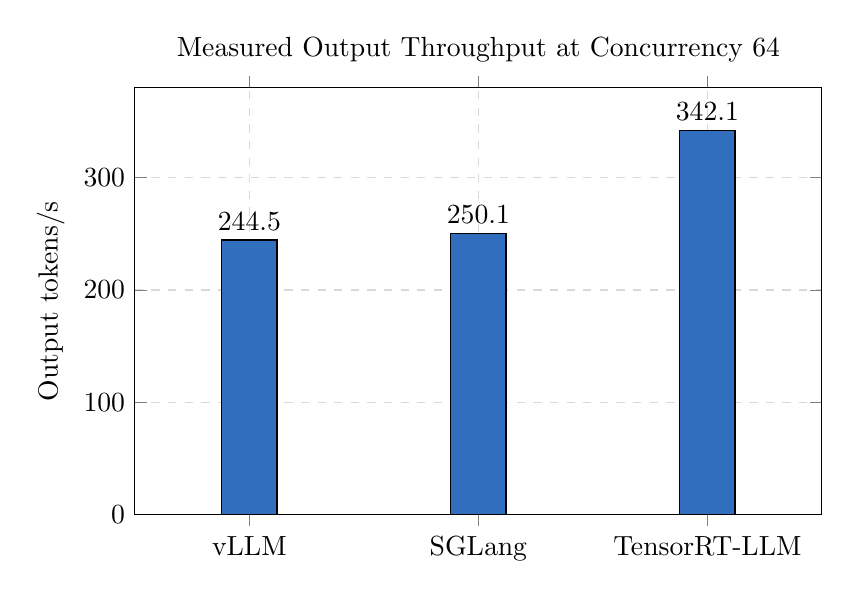
\begin{tikzpicture}
\begin{axis}[
    ybar,
    bar width=20pt,
    width=0.85\textwidth,
    height=7cm,
    ylabel={Output tokens/s},
    symbolic x coords={vLLM,SGLang,TensorRT-LLM},
    xtick=data,
    ymin=0,
    ymax=380,
    nodes near coords,
    nodes near coords align={vertical},
    grid=major,
    grid style={dashed,gray!30},
    title={Measured Output Throughput at Concurrency 64},
    enlarge x limits=0.25
]
\addplot[
    fill=gpuBlue
] coordinates {
    (vLLM,244.5)
    (SGLang,250.1)
    (TensorRT-LLM,342.1)
};
\end{axis}
\end{tikzpicture}

\caption{Output-token throughput from a single-GPU Qwen3-32B-FP8
benchmark.}
\end{figure}

% ============================================================
\section{Measured Time to First Token}
% ============================================================

For the same benchmark at concurrency 8:

\[
\begin{array}{l|r}
\text{Framework} & \text{Average TTFT (ms)}\\
\hline
\text{vLLM} & 834\\
\text{SGLang} & 2029\\
\text{TensorRT-LLM} & 2541
\end{array}
\]

At concurrency 32:

\[
\begin{array}{l|r}
\text{Framework} & \text{Average TTFT (ms)}\\
\hline
\text{vLLM} & 11125\\
\text{SGLang} & 12332\\
\text{TensorRT-LLM} & 4554
\end{array}
\]

At concurrency 64:

\[
\begin{array}{l|r}
\text{Framework} & \text{Average TTFT (ms)}\\
\hline
\text{vLLM} & 40565\\
\text{SGLang} & 40601\\
\text{TensorRT-LLM} & 11738
\end{array}
\]

The result demonstrates why one-dimensional ``fastest framework''
rankings are misleading: the latency relationship changes as
concurrency changes \cite{benchmark2026}.

\begin{figure}[H]
\centering

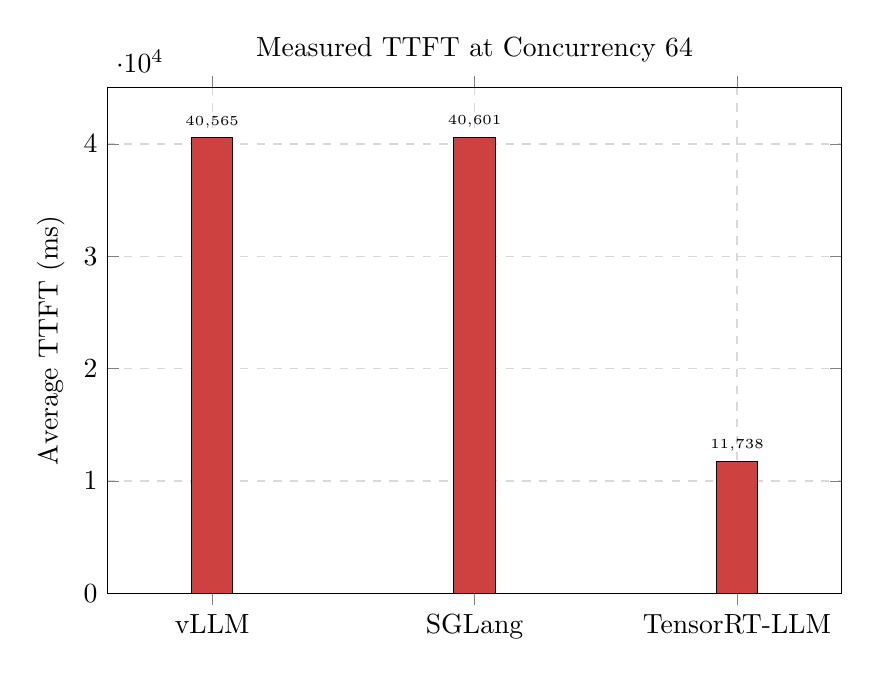
\begin{tikzpicture}
\begin{axis}[
    ybar,
    bar width=15pt,
    width=0.9\textwidth,
    height=8cm,
    ylabel={Average TTFT (ms)},
    symbolic x coords={vLLM,SGLang,TensorRT-LLM},
    xtick=data,
    ymin=0,
    ymax=45000,
    nodes near coords,
    nodes near coords style={font=\tiny},
    grid=major,
    grid style={dashed,gray!30},
    title={Measured TTFT at Concurrency 64},
    enlarge x limits=0.2
]
\addplot[
    fill=latencyRed
] coordinates {
    (vLLM,40565)
    (SGLang,40601)
    (TensorRT-LLM,11738)
};
\end{axis}
\end{tikzpicture}

\caption{Average time to first token at concurrency 64.}
\end{figure}

% ============================================================
\section{Long-Context Behavior}
% ============================================================

The same benchmark also tested:

\[
I=8000,\qquad O=512,\qquad C=8.
\]

Reported output throughput:

\[
\begin{array}{l|r}
\text{Framework} & \text{Output tokens/s}\\
\hline
\text{vLLM} & 41.0\\
\text{SGLang} & 38.2\\
\text{TensorRT-LLM} & 75.9
\end{array}
\]

Reported average TTFT:

\[
\begin{array}{l|r}
\text{Framework} & \text{TTFT (ms)}\\
\hline
\text{vLLM} & 63824\\
\text{SGLang} & 68593\\
\text{TensorRT-LLM} & 8560
\end{array}
\]

This illustrates the importance of testing the actual workload rather
than extrapolating from short prompts.

% ============================================================
\section{Energy Per Token}
% ============================================================

\subsection{Definition}

The most useful metric for the user's energy-efficiency question is

\[
\boxed{
E_{\mathrm{token}}
=
\frac{E_{\mathrm{inference}}}
{N_{\mathrm{output\ tokens}}}
}
\]

with units

\[
[E_{\mathrm{token}}]
=
\mathrm{J/token}.
\]

Equivalently,

\[
\boxed{
\eta_{\mathrm{token}}
=
\frac{N_{\mathrm{output\ tokens}}}
{E_{\mathrm{inference}}}
}
\]

has units

\[
\mathrm{tokens/J}.
\]

The relationship is

\[
E_{\mathrm{token}}
=
\frac{1}{\eta_{\mathrm{token}}}.
\]

\subsection{Power-Based Measurement}

If instantaneous power is measured as $P(t)$, then

\[
E
=
\int_{t_0}^{t_1}P(t)\,dt.
\]

Therefore,

\[
\boxed{
E_{\mathrm{token}}
=
\frac{
\int_{t_0}^{t_1}P(t)\,dt
}{
N_{\mathrm{output}}
}
}
\]

For approximately constant power,

\[
E_{\mathrm{token}}
\approx
\frac{P\Delta t}
{N_{\mathrm{output}}}.
\]

Since

\[
R_{\mathrm{token}}
=
\frac{N_{\mathrm{output}}}{\Delta t},
\]

we obtain

\[
\boxed{
E_{\mathrm{token}}
\approx
\frac{P}{R_{\mathrm{token}}}
}
\]

which provides a very useful connection between power and throughput.

% ============================================================
\section{Energy--Throughput Relationship}
% ============================================================

Suppose a framework produces

\[
R=300\ \tokps
\]

while consuming

\[
P=300\ \mathrm{W}.
\]

Then

\[
E_{\mathrm{token}}
=
\frac{300}{300}
=
1\ \jptok.
\]

If another runtime produces

\[
R=400\ \tokps
\]

at

\[
P=360\ \mathrm{W},
\]

then

\[
E_{\mathrm{token}}
=
\frac{360}{400}
=
0.9\ \jptok.
\]

The second system therefore uses more total power but less energy
per generated token.

This is why:

\[
\boxed{
\text{minimum power}
\neq
\text{minimum energy/token}
}
\]

and

\[
\boxed{
\text{maximum tokens/s}
\neq
\text{maximum tokens/J}.
}
\]

% ============================================================
\section{Energy Efficiency Graph Template}
% ============================================================

The ideal comparison graph places:

\[
x=\text{output tokens/s}
\]

and

\[
y=\mathrm{J/token}.
\]

The desirable region is:

\[
\boxed{
x\rightarrow\text{large},
\qquad
y\rightarrow\text{small}.
}
\]

Because comparable public power measurements are not available for
all 24 systems in the benchmark used here, the following plot is
deliberately a \emph{measurement template} rather than fabricated
framework data.

\begin{figure}[H]
\centering

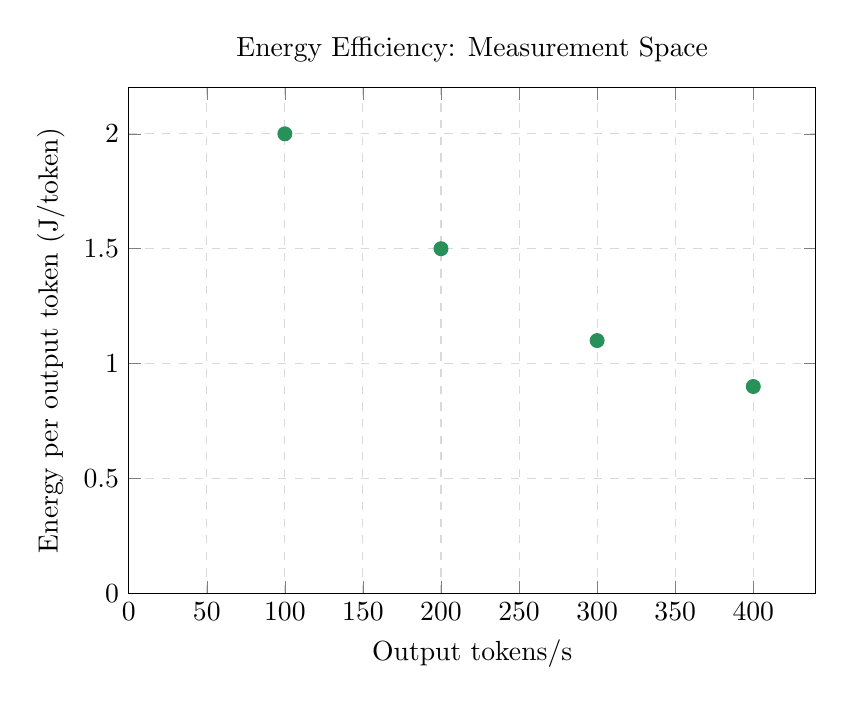
\begin{tikzpicture}
\begin{axis}[
    width=0.85\textwidth,
    height=8cm,
    xlabel={Output tokens/s},
    ylabel={Energy per output token (J/token)},
    xmin=0,
    ymin=0,
    grid=major,
    grid style={dashed,gray!30},
    title={Energy Efficiency: Measurement Space},
]

% Illustrative measurement points ONLY
\addplot[
    only marks,
    mark=*,
    mark size=2.5pt,
    color=energyGreen
] coordinates {
    (100,2.0)
    (200,1.5)
    (300,1.1)
    (400,0.9)
};

\end{axis}
\end{tikzpicture}

\caption{
Illustrative geometry of an energy-throughput comparison.
The points are not framework measurements and are included only to
show the desired measurement space.
}
\end{figure}

% ============================================================
\section{Recommended Energy Benchmark Protocol}
% ============================================================

A reproducible experiment should record:

\begin{table}[H]
\centering
\begin{tabular}{ll}
\toprule
Parameter & Required value \\
\midrule
Model & Exact model identifier \\
Hardware & Exact GPU/CPU/NPU model \\
Precision & FP16/BF16/FP8/INT8/INT4/etc. \\
Input tokens & Fixed or distribution specified \\
Output tokens & Fixed or distribution specified \\
Concurrency & Fixed sweep \\
Batching & Enabled/disabled and configuration \\
Power limit & Explicit value \\
Ambient temperature & Recorded \\
Driver & Version recorded \\
Runtime & Exact commit/version \\
CUDA/ROCm/Metal & Exact version \\
Warm-up & Explicit number of iterations \\
Measurement interval & Explicit sampling frequency \\
Energy boundary & GPU only / system / wall power \\
\bottomrule
\end{tabular}
\caption{Minimum metadata for an energy benchmark.}
\end{table}

The experiment should measure at least:

\[
\left\{
P(t),
T,
N_{\mathrm{input}},
N_{\mathrm{output}},
\mathrm{TTFT},
\mathrm{ITL},
\mathrm{throughput}
\right\}.
\]

Then calculate

\[
E_{\mathrm{GPU}}
=
\int P_{\mathrm{GPU}}(t)\,dt,
\]

and

\[
E_{\mathrm{system}}
=
\int P_{\mathrm{wall}}(t)\,dt,
\]

where $P_{\mathrm{GPU}}$ is measured at the GPU power rails and
$P_{\mathrm{wall}}$ at the wall outlet.

The resulting energy per token is then

\[
\boxed{
E_{\mathrm{token}}
=
\frac{
\int_{t_0}^{t_1}P_{\mathrm{GPU}}(t)\,dt
+
\int_{t_0}^{t_1}P_{\mathrm{CPU}}(t)\,dt
}{
N_{\mathrm{output}}
}
}
\]

or, for a system-level answer,

\[
\boxed{
E_{\mathrm{token,wall}}
=
\frac{
\int_{t_0}^{t_1}P_{\mathrm{wall}}(t)\,dt
}{
N_{\mathrm{output}}
}
}
\]

depending on whether the experiment boundary is the accelerator or
the whole machine.

% ============================================================
\section{Conclusion}
% ============================================================

Modern AI inference performance is determined by the interplay of
the model, the runtime, the hardware, and the workload, not by any
single framework in isolation.

The main takeaways are:

\begin{enumerate}
    \item Reported token throughput and TTFT are workload- and
    hardware-specific measurements, not immutable framework
    properties \cite{benchmark2026}.
    \item Energy efficiency must be measured as joules per generated
    token at a defined power boundary (GPU rail vs.\ wall).
    \item A framework that maximizes tokens/s is not guaranteed to
    minimize J/token, because total power also changes.
    \item Reliable comparisons require the metadata listed in the
    Recommended Energy Benchmark Protocol above.
\end{enumerate}

No single framework is universally optimal.  The correct choice
depends on the model, hardware, serving traffic, quantization, and
latency targets for the specific deployment.

\begin{thebibliography}{9}

\bibitem{benchmark2026}
Qwen3-32B FP8 single-GPU serving benchmark: output-token throughput
and time-to-first-token for vLLM, SGLang, and TensorRT-LLM across
concurrencies and context lengths, 2026.

\end{thebibliography}

\end{document}
\[
